\documentclass{beamer}
\usepackage{amsmath}
\usepackage[utf8]{inputenc}
\usepackage{graphics}
\usepackage{hyperref}
\usepackage{xcolor}
\usepackage{wasysym}
\usepackage{listings}
\usepackage{tikz}
\usepackage{amssymb}
\usepackage[normalem]{ulem}
\usepackage{textcomp}
\usepackage{verbatim}
\usepackage[T1]{fontenc}
\usepackage{lmodern}
\usetikzlibrary{shapes.callouts,shadows, calc}

\tikzset{note/.style={rectangle callout, rounded corners,fill=gray!20,drop shadow,font=\footnotesize}}    
\newcommand{\tikzmark}[1]{\tikz[overlay,remember picture] \node (#1) {};}    

\newcounter{image}
\setcounter{image}{1}

\makeatletter
\newenvironment{btHighlight}[1][]
{\begingroup\tikzset{bt@Highlight@par/.style={#1}}\begin{lrbox}{\@tempboxa}}
{\end{lrbox}\bt@HL@box[bt@Highlight@par]{\@tempboxa}\endgroup}

\newcommand\btHL[1][]{%
  \begin{btHighlight}[#1]\bgroup\aftergroup\bt@HL@endenv%
}
\def\bt@HL@endenv{%
  \end{btHighlight}%   
  \egroup
}
\newcommand{\bt@HL@box}[2][]{%
  \tikz[#1]{%
    \pgfpathrectangle{\pgfpoint{0pt}{0pt}}{\pgfpoint{\wd #2}{\ht #2}}%
    \pgfusepath{use as bounding box}%
    \node[anchor=base west,rounded corners, fill=green!30,outer sep=0pt,inner xsep=0.2em, inner ysep=0.1em,  #1](a\theimage){\usebox{#2}};
  }%
 \stepcounter{image}
}
\makeatother

\usetheme{Warsaw}
\usecolortheme{lily}
\setbeamercovered{transparent}
\setbeamertemplate{headline}{
  \begin{beamercolorbox}{section in head/foot}
    \vskip2pt\insertnavigation{\paperwidth}\vskip2pt
  \end{beamercolorbox}
}

\setbeamertemplate{footline}{
}

\author{
  {\tiny Tony Morris\\}
}

\xdefinecolor{darkgreen}{rgb}{0,0.35,0}
\lstset{
  tabsize=2,
  basicstyle=\ttfamily,
  moredelim=**[is][\btHL]{`}{`}
}
\lstdefinestyle{java}{
  language=java,
  basicstyle=\footnotesize\ttfamily,
  stringstyle=\color{darkgreen}\ttfamily,
  commentstyle=\color{gray}\ttfamily,
  keywordstyle=\footnotesize\color{blue}\ttfamily,
  tabsize=2,
  moredelim=**[is][\btHL]{`}{`}
}
\lstdefinelanguage{scala}{
  morekeywords={abstract,case,catch,class,def,%
    do,else,extends,false,final,finally,%
    for,forSome,if,implicit,import,lazy,match,%
    new,null,object,override,package,%
    private,protected,requires,return,sealed,%
    super,this,throw,trait,true,try,%
    type,val,var,while,with,yield},
  otherkeywords={=,=>,<-,<\%,<:,>:,\#,@},
  sensitive=true,
  morecomment=[l]{//},
  morecomment=[n]{/*}{*/},
  morestring=[b]",
  morestring=[b]',
  morestring=[b]"""
}
\lstdefinelanguage{haskell}{
  morekeywords={class,instance,where,do,data,newtype,default,deriving,module},
  otherkeywords={<-},
  sensitive=true,
  morecomment=[l]{--},
  morecomment=[n]{\{-}{-\}}, 
  morestring=[b]",
  morestring=[b]',
  morestring=[b]"""
}
\lstdefinestyle{scala}{
  language=scala,
  basicstyle=\footnotesize\ttfamily,
  stringstyle=\color{darkgreen}\ttfamily,
  commentstyle=\color{gray}\ttfamily,
  keywordstyle=\footnotesize\color{blue}\ttfamily,
  tabsize=2,
  moredelim=**[is][\btHL]{`}{`}
}
\lstdefinestyle{haskell}{
  language=haskell,
  basicstyle=\tiny\ttfamily,
  stringstyle=\color{darkgreen}\ttfamily,
  commentstyle=\color{gray}\ttfamily,
  keywordstyle=\tiny\color{blue}\ttfamily,
  tabsize=2
}
% #866eaa
\definecolor{nicta-purple}{rgb}{0.5234,0.4297,0.6640}

\defbeamertemplate*{title page}{customized}[1][] {
  \centering
  \color{nicta-purple}
  \usebeamerfont{title}\inserttitle\par
  \bigskip
  \usebeamerfont{subtitle}\insertsubtitle\par
  \bigskip
  \bigskip
  \bigskip
  \bigskip
  \usebeamerfont{institute}\insertinstitute\par
  \bigskip
  \usebeamerfont{author}\insertauthor\par
  % \usebeamerfont{date}\insertdate\par
  \usebeamercolor[fg]{titlegraphic}\inserttitlegraphic
}

\logo{
\includegraphics[height=0.8cm]{image/nicta.jpg}}

\begin{document}
\title{\large The Essential Tools of Open-Source}
\subtitle{\tiny Functional Programming, Parametricity, Types}
\institute[NICTA]{}
\date {
  lca2016 FP Miniconf, 02 February 2016
}

\normalsize

\setbeamercovered{transparent}
\begin{frame}
  \titlepage
\end{frame}

\begin{frame}
\frametitle{The Claim}
\begin{block}{the following are essential to success\ldots}
\begin{itemize}
\item<1-> adherence to the functional programming thesis
\item<2-> parametricity (and types)
\end{itemize}
\end{block}
\end{frame}

\begin{frame}[fragile]
\frametitle{The Parametricity Trick}
\begin{block}{parametricity will only work with\ldots}
\begin{itemize}
\item<1-> an inveterate exploitation of the functional programming thesis
\item<2-> let's revisit functional programming
\end{itemize}
\end{block}
\end{frame}

\begin{frame}
\frametitle{Reminder}
\begin{block}{so what is functional programming?}
\begin{itemize}
\item<1-> a means of programming by which expressions are \emph{referentially transparent}.
\item<2-> but what is referential transparency?
\end{itemize}
\end{block}
\end{frame}

\begin{frame}
\frametitle{Referential Transparency}
\begin{itemize}
  \item<1> referential transparency is a decidable property of expressions
  \item<2> functions provide programmers a tool to create referentially transparent expressions
\end{itemize}
\begin{block}<3>{The Test for Referential Transparency}
An expression \lstinline$expr$ is referentially transparent if in a program \lstinline$p$, all occurrences of \lstinline$expr$ in \lstinline$p$ can be replaced by an assignment to \lstinline$expr$ without effecting an observable change in \lstinline$p$.
\end{block}
\end{frame}

\begin{frame}[fragile]
\frametitle{Referential Transparency}
\begin{block}<1>{Example program}
\begin{lstlisting}
p = {
  r = buffer.append(x)
  r = buffer.append(x)
  f(r, r)
}
\end{lstlisting}
\end{block}
\begin{block}<2>{Refactoring of program}
\begin{lstlisting}
p = {
  f(buffer.append(x), buffer.append(x))
}
\end{lstlisting}
\end{block}
\begin{block}<3>{}
Is the program refactoring observable for all values of \lstinline$f$?
\end{block}
\end{frame}

\begin{frame}[fragile]
\frametitle{Referential Transparency}
\begin{block}<1>{Example program}
\begin{lstlisting}
p = {
  r = str.length()
  r = str.length()
  f(r, r)
}
\end{lstlisting}
\end{block}
\begin{block}<2>{Refactoring of program}
\begin{lstlisting}
p = {
  f(str.length(), str.length())
}
\end{lstlisting}
\end{block}
\begin{block}<3>{}
Is the program refactoring observable for all values of \lstinline$f$?
\end{block}
\end{frame}

\begin{frame}
\frametitle{Functional Programming}
\begin{itemize}
  \item<1> FP is a commitment to preserving referential transparency
  \item<2> FP has won by not-a-little-bit. FP is essential. Moving on.
  \item<3> we use tools to achieve this commitment
  \item<4> parametricity is one such tool with high reward
\end{itemize}
\end{frame}

\begin{frame}
\frametitle{What is Parametricity}
\begin{block}{Danielsson, Hughes, Jansson \& Gibbons \cite{danielsson2006fast} tell us:}
\begin{quotation}
Functional programmers often reason about programs as if
they were written in a total language, expecting the results
to carry over to non-total (partial) languages. We justify
such reasoning.
\end{quotation}
\end{block}
\end{frame}

\begin{frame}
\frametitle{What is Parametricity}
\begin{block}{Philip Wadler \cite{wadler1989theorems} tells us:}
\begin{quotation}
Write down the definition of a polymorphic function on a piece of paper. Tell me its type, but be careful not to let me see the function's definition. I will tell you a theorem that the function satisfies.

The purpose of this paper is to explain the trick.
\end{quotation}
\end{block}
\end{frame}

\begin{frame}[fragile]
\frametitle{Types}
\begin{block}{first let's talk about types}
Suppose we encountered the following function definition:
\begin{lstlisting}
int add12(int)
\end{lstlisting}
\end{block}
\begin{itemize}
  \item<1> by the type alone, there are {$({2^{32}})^{2^{32}}$} possible implementations
  \item<2> but this is a significantly smaller number than \rotatebox{90}{8}
\end{itemize}
\end{frame}

\begin{frame}[fragile]
\frametitle{Types}
\framesubtitle{reading the code}
We might form a suspicion that \lstinline[style=scala]$add12$ adds twelve to its argument
\begin{lstlisting}[style=scala]
int `add12`(int)
\end{lstlisting}
\begin{tikzpicture}[remember picture,overlay]
\coordinate (aa) at ($(a1)+(7,2.0)$);
\node[note,draw,callout relative pointer={($(aa)-(11.2,-3.7)$)},right] at (aa) {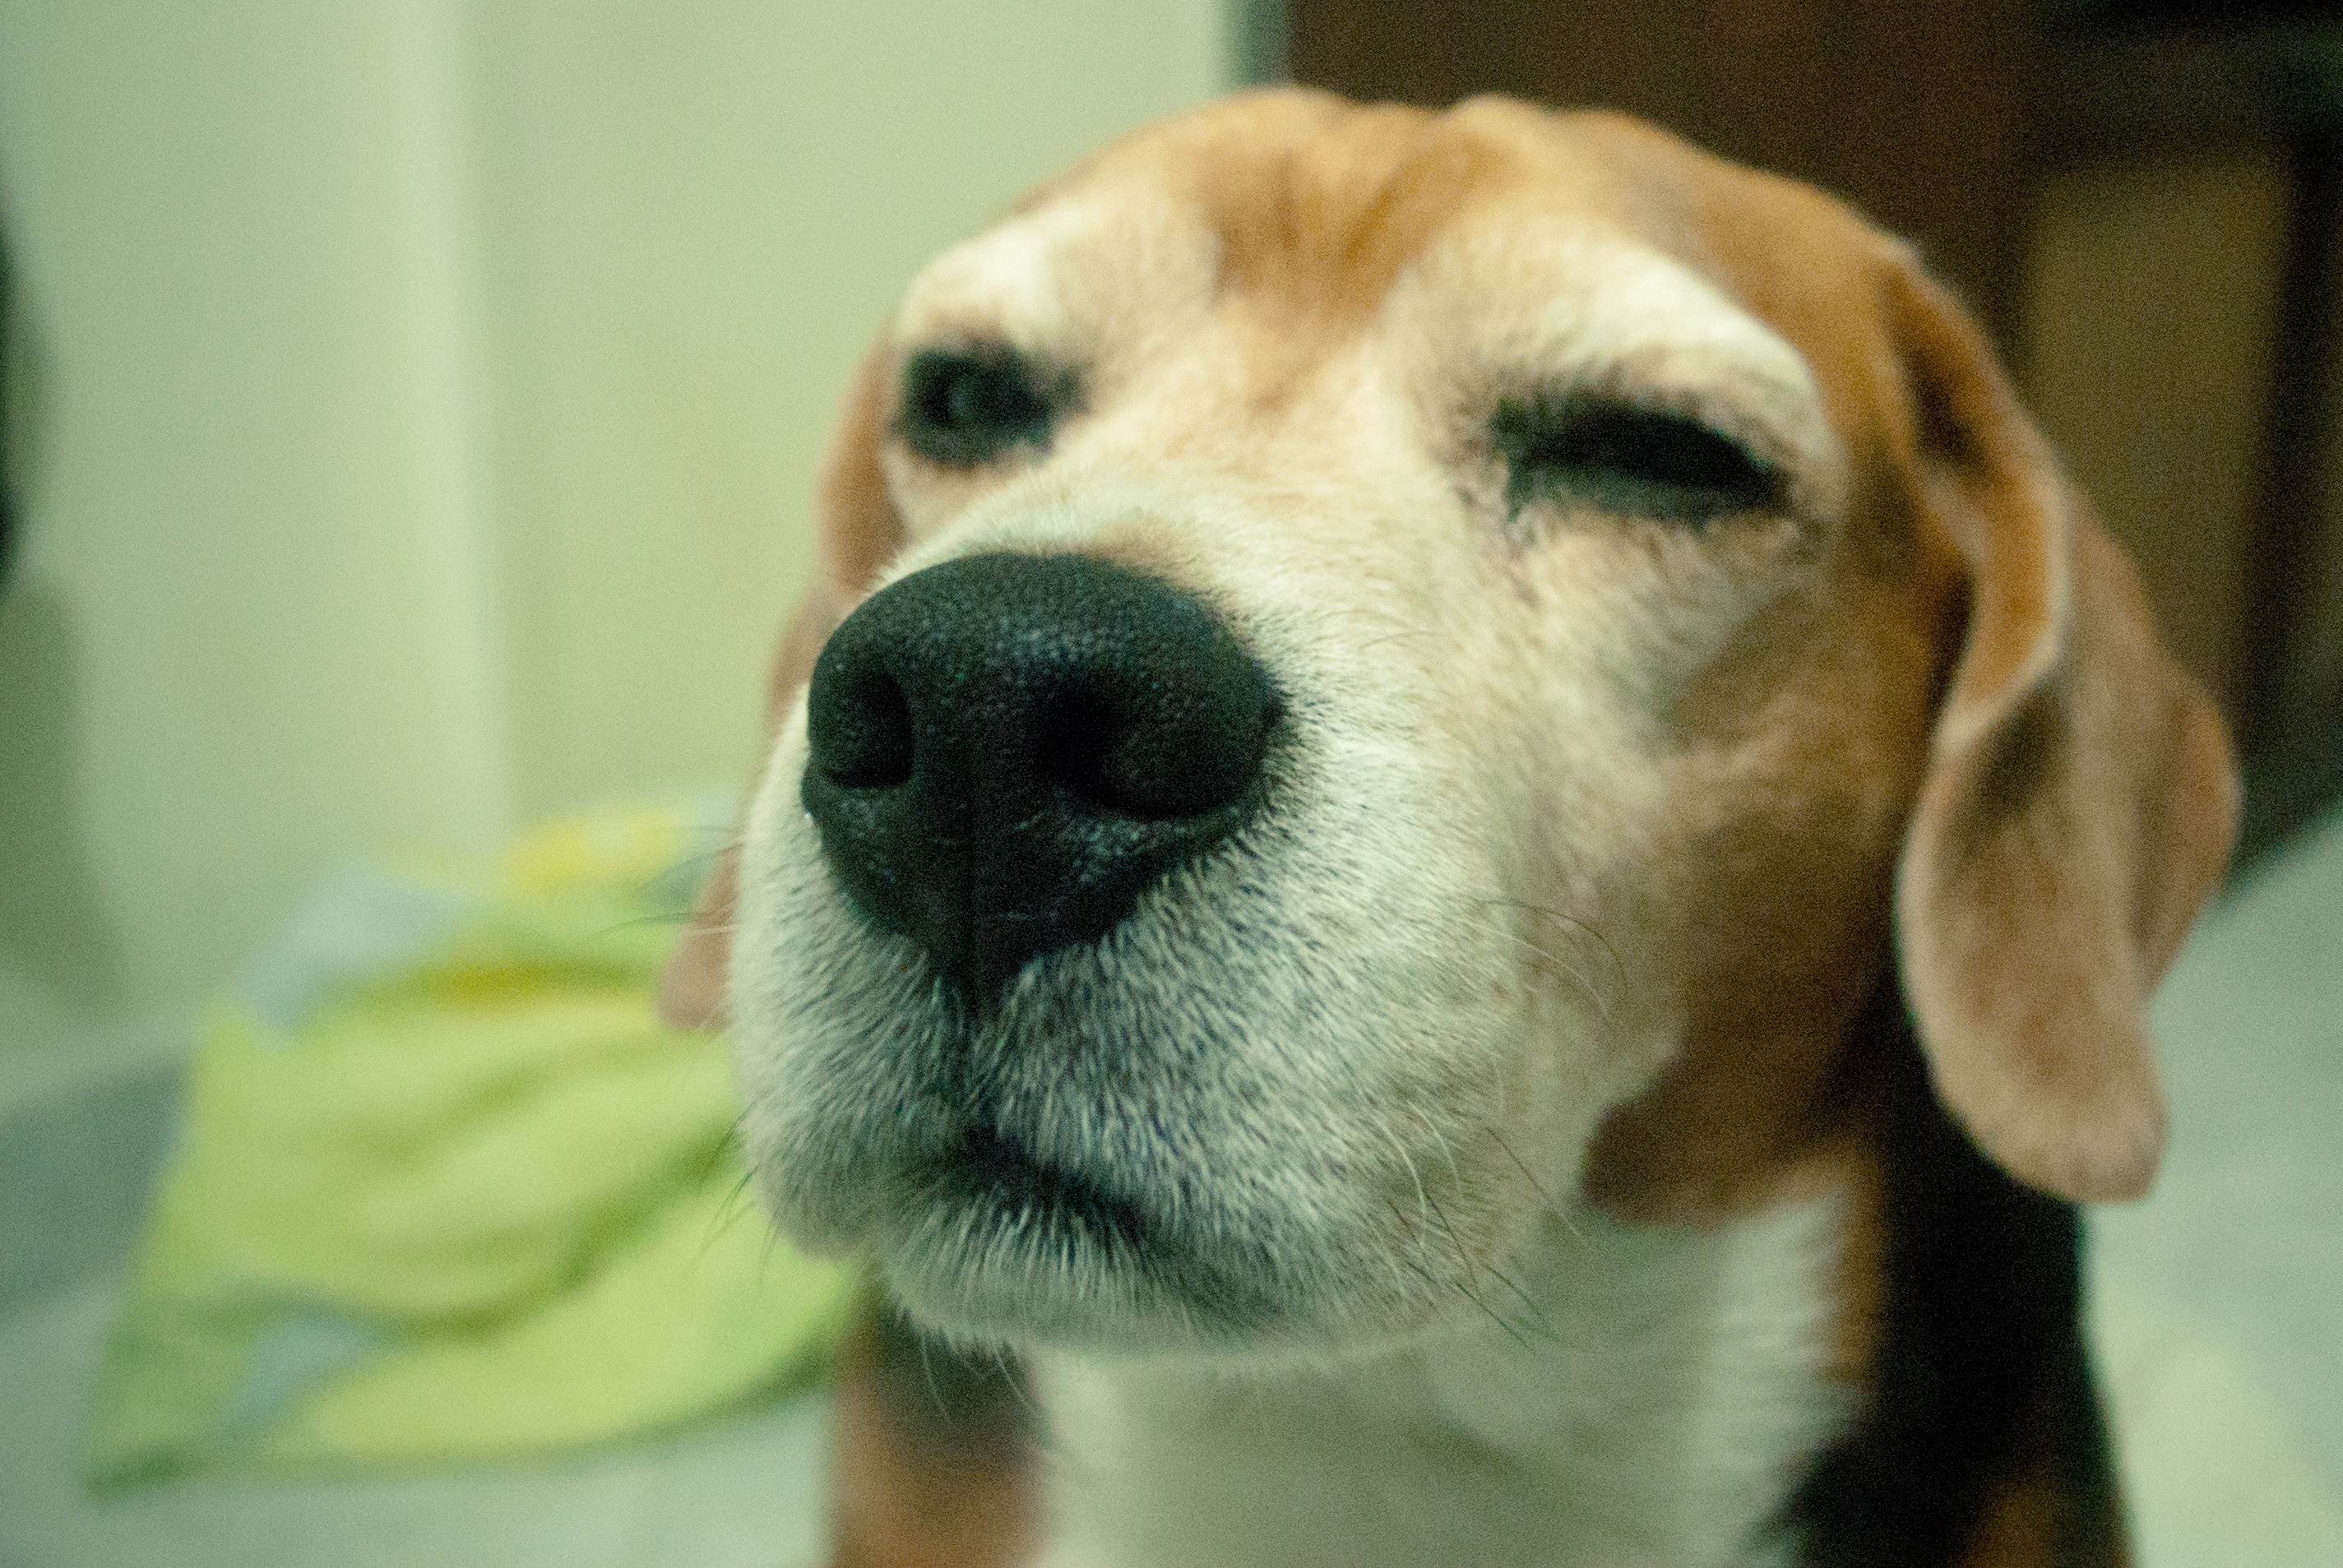
\includegraphics[width=0.2\textwidth]{image/suspicion.jpg}};
\end{tikzpicture}
\end{frame}

\begin{frame}[fragile]
\frametitle{Types}
So we write some tests:
\begin{lstlisting}
add12(0)        = 12
add12(5)        = 17
add12(-5)       = 7
add12(223)      = 235
add12(5096)     = 5104
add12(2914578)  = 29145590
add12(-2914578) = -29145566
\end{lstlisting}
And conclude, yes, this function adds twelve to its argument
\end{frame}

\begin{frame}[fragile]
\frametitle{Types}
\framesubtitle{Woops!}
\begin{lstlisting}
def add12(n: Int): Int =
  if(n < 8000000) n + 12
  else n * 7
\end{lstlisting}
Narrowing the potential propositions about what this function does not do.
\end{frame}

\begin{frame}[fragile]
\frametitle{Types}
\begin{block}{another monomorphic example}
\begin{lstlisting}
List<int> function(List<int>)
\end{lstlisting}
\end{block}
\begin{itemize}
  \item<1> adds 17 to every 11th element?
  \item<2> drops every prime number?
\end{itemize}
\end{frame}

\begin{frame}[fragile]
\frametitle{Parametricity}
\begin{block}{a polymorphic example}
\begin{lstlisting}
<A> List<A> function(List<A>)
\end{lstlisting}
\end{block}
\begin{itemize}
  \item<1> this function returns elements in a list that always appear in the argument
  \item<2> this function never inspects the elements, only rearranges them
\end{itemize}
\end{frame}

\begin{frame}[fragile]
\frametitle{Parametricity}
\begin{block}{the goal}
\begin{itemize}
  \item<1> a significant number of possible things that this function does are eliminated, by no expenditure of effort.
  \item<2> theorems about this function can be reliably constructed
\end{itemize}
\end{block}
\end{frame}

\begin{frame}[fragile]
\frametitle{Reasoning with parametricity}
\begin{block}{Fast and loose reasoning is morally correct \cite{danielsson2006fast}}
\small{Functional programmers often reason about programs as if
they were written in a total language, expecting the results
to carry over to non-total (partial) languages. We justify
such reasoning.}
\end{block}
but what does this mean exactly?
\end{frame}


\begin{frame}[fragile]
\frametitle{Fast and Loose Reasoning}
\begin{lstlisting}
boolean even(int i) =
  ...
\end{lstlisting}
This function returns one of two things.
\end{frame}

\begin{frame}[fragile]
\frametitle{Fast and Loose Reasoning}
\begin{lstlisting}
boolean even(int i) =
  even(i)
\end{lstlisting}
and we can discard this third possibility in analysis.
\end{frame}

\begin{frame}[fragile]
\frametitle{Fast and Loose Reasoning}
\begin{block}{many programming environments involve}
\begin{itemize}
  \item \lstinline{null}
  \item exceptions
  \item Type-casing
  \item Type-casting
  \item Side-effects \footnote{but FP has won}
  \item universal \lstinline{equals}/\lstinline{toString}
\end{itemize}
\end{block}
These must \emph{all be discarded}.
\end{frame}


\begin{frame}[fragile]
\frametitle{The Limits of Parametricity}
\begin{lstlisting}
<A> List<A> function(List<A>)
\end{lstlisting}
OK, so we know that all elements in the result appear in the input
\begin{itemize}
  \item convince yourself of this fact
  \item but how do we narrow it down?
  \item how do we rule out all possibilities for the type but one?
  \item how do we unambiguously determine what the function does?
\end{itemize}
\end{frame}

\begin{frame}[fragile]
\frametitle{The Limits of Parametricity}
\begin{block}{what does this function do?}
\lstinputlisting[style=haskell]{source/reverse-with-tests.hs}
\end{block}
\end{frame}

\begin{frame}[fragile]
\frametitle{Once-inhabitance}
\begin{block}{sometimes tests are unnecessary}
\begin{lstlisting}[style=haskell]
f :: a -> a
\end{lstlisting}
\end{block}
\end{frame}

\begin{frame}[fragile]
\frametitle{Once-inhabitance}
\begin{block}{sometimes tests are unnecessary}
\begin{lstlisting}[style=haskell]
g :: Functor f => y -> f x -> f y
\end{lstlisting}
\end{block}
\begin{lstlisting}[style=haskell]
> g "hi" [1,2,3]
["hi","hi","hi"]
\end{lstlisting}
\end{frame}

\begin{frame}[fragile]
\frametitle{Parametricity}
\begin{block}{non-trivial example}
\begin{lstlisting}[style=haskell]
both ::
  (Applicative f, Bitraversable r) =>
  (a -> f b) -> r a a -> f (r b b)
\end{lstlisting}
\end{block}
\tiny
\begin{itemize}
  \item<1-> This function can only \lstinline{bitraverse} \footnote{(and derivatives)} on \lstinline{(`r`)}
  \begin{itemize}
    \item \tiny{will work with \lstinline{Either} at call site}
    \item \tiny{will work with \lstinline{(,)} at call site}
    \item \tiny{will work with \lstinline{Const} at call site}
    \item \tiny{\textbf{but \lstinline{both} cannot do anything specific to these data types}}
  \end{itemize}
  \item<2-> This function can only \lstinline{(<*>)} and \lstinline{pure} on \lstinline{(`f`)}
  \begin{itemize}
    \item \tiny{will work with \lstinline{Maybe} at call site}
    \item \tiny{will work with \lstinline{IO} at call site}
    \item \tiny{e.g. call site can open network connections using \lstinline{both}}
    \item \tiny{\textbf{however \lstinline{both} definitely does not open any network connections itself}}
  \end{itemize}
  \item<3-> \lstinline{(`a`)} and \lstinline{(`b`)} might be anything
  \begin{itemize}
    \item \tiny{may be \lstinline{Int} at call site}
    \item \tiny{may be \lstinline{String} at call site}
    \item \tiny{\textbf{however \lstinline{both} definitely does not perform any \lstinline{Int}-specific operations}}
  \end{itemize}
\end{itemize}
\end{frame}

\begin{frame}[fragile]
\frametitle{Parametricity}
\begin{block}{and on it goes}
\begin{lstlisting}[style=haskell]
(<.) ::
  Indexable i p =>
  (Indexed i s t -> r) -> ((a -> b) -> s -> t) -> p a b -> r
\end{lstlisting}
\end{block}
\end{frame}

\begin{frame}[fragile]
\frametitle{Parametricity and open-source}
\begin{block}{my open-source goals}
\begin{itemize}
  \item can fix bugs independently of the possibility of creating more
  \item can introduce features without adversely affecting others
  \item can have hundreds of projects requiring zero maintenance
  \item \textbf{avoid endless tail-chasing that prevails in corporate dev}
\end{itemize}
\end{block}
\end{frame}

\begin{frame}[fragile]
\frametitle{Parametricity and open-source}
\begin{block}{Department of Defense 29 January 2016}
\begin{quotation}
The Marine Corps' F-35B aircraft are being delivered with Block 2B software, which Gilmore said has "hundreds of unresolved deficiencies." And those problems have compounded in Block 3F software. That's because the first round of Block 3 was created by "re-hosting the immature Block 2B software…into new processors to create Block 3i," the initial release for the code, Gilmore noted. This led to "avionics instabilities and other new problems, resulting in poor performance during developmental testing."
\end{quotation}
\end{block}
\end{frame}


\begin{frame}[fragile]
\frametitle{Parametricity and open-source}
\begin{block}{goals}
The value of parametricity is too high to forgo in open-source development. And for what possible benefit?
\end{block}
\end{frame}

\begin{frame}[fragile]
\frametitle{Parametricity and open-source}
\begin{block}{goals}
\begin{itemize}
  \item what's it like for you haskell programmers in the ivory tower?
  \item why are you so averse to programming language environment X?
\end{itemize}
\end{block}
\end{frame}

\begin{frame}
\frametitle{References}

\bibliographystyle{amsalpha}
\bibliography{parametricity}

\end{frame}


\end{document}
